\section{The greedy algorithm}
\subsection{Description of greedy algorithms.}
Greedy algorithms can be either iterative or recursive. Any problem that can be solved recursively can also be solved iteratively \cite{recursion}. For simplicity we will consider the greedy algorithms as being iterative unless stated otherwice. In each iteration the algorithm has a set of possible alternatives on how to to push the algorithm towards a solution. A cost function designates a cost to each alternative. At the end of the iteration the alternative with the best cost, be it maximum or minimun, is choosen as a part of the solution. \\
\\There is no general way of determining whether a greedy algorithm provides an optimal solution or not, but there are two very important properties that usually helps to determine if an optimal solution can be provided. These are the greedy-choice property and the optimal substructure property \cite{introduction to Algorithms}. The greedy choice property states that an global optimal solution can be arrived at by making locally optimal choices. In other words, at each iteration a choice can be made without reconsidering previous iterations. The optimal substructure property states that the problem can be divided into subproblems, which each have an optimal solution. If these two properties are fullfilled, then a solution can be constructed by the optimal subsolutions. Hopefully this is an optimal solution, but if one want's to be certain more rigorous proofs are needed. 

\subsection{Development process for the greedy algorithm.}
When constructing a greedy algorithm one often starts by finding some part of the final solution and then extend this to find a correct generic question for recursion. As in the examples given in the online lectures \cite{online lecture} the question and answer yielding a correct algorithm may not be intuitive. In the approach of creating the greedy algorithm for our problem we assume that it is possible to find the best movement strategy by locally finding the best next step until the enviroment has been secured. So the generic question would informally be "what is the best next step for the pursuer team?". In the development process for the greedy algorithm there have been a couple of candidates on how to answer this question. At last only one seemed like a good choice, presented in Section 4.1.3.\\
\\The first candidate "alorithm 1" was to make the secured area our objective function. In each iteration we consider the next move for each pursuer in the team, and try to move the whole group so that we maximize the secured area (the objective function). We would then have an objective function and constraints that depend on the enviroment and pursuer positions. The idea was to try and formulate this as a linear programming problem, since there exists a lot of framework for solving linear programming problems. After consideration this naive approach presented several drawbacks. First off, for many enviroments it is sometimes nessecary to let go of secured areas \cite{guidas}. This could not be alowed by algorithm 1 with a greedy approach. Also there are a lot of cases where the best move is not an increase in secured area, but rather guarding or transportation to strategic positions. This was allowed, but not very likely to be chosen by the algorithm due to the greedy approach. It was thus realized that the algorithm somehow must look further than just the head on approach of targeting the secured area.\\
\\The next candidate was an attempt to extend the formulation of algorithm 1 to have dynamic constraints, hereon called algorithm 2. The idea was to introduce some sort of tactics to the pursuer team, and thus make the group cooperate in a favorable manor. For each pursuer a certain tactic would be given, corresponding to constraints to optimization problem. In order to formulate these constraints, we needed more information. Here the idea of introducing different areas was first met. The common vision of the pursuer team divides the enviroment into several subareas, not visible by the team. Depending on the state and geometry of these subareas each pursuer was supposed to either guard, secure or divide a given subarea. This is dynamic information about the enviroment, thus giving dynamic constraints for each pursuer. In this case it was problematic to find a general formulation of how to choose a tactic, and how to formulate these tactics as constraints for the objective function. Also there were to many special cases and intuition involved for a possible implementation.\\
\\For the third candidate "algorithm 3" the idea was to use the extra enviromental information about the non visible areas and somehow apply this to a simple greedy cost function. By designating costs to each feasible tile it would be easy to make a greedy choice. By construction each hunter can in general move to at most four tiles or stand still. Thus by giving each of these five alternatives a value that quantifies how good the move is we'll find the best over all strategy of the team. With this setup the objective function for each itteration is to maximize the sum of the tile-values that each pursuer moves into. So, how does one quantify what  a good tile is? The obvious answers such as field of vision and state are, by them self, insufficent information for a good algorithm. But by using the dynamic information of the areas, resulting from the pursuers vision, we can find more parameters to quantify the best move. In order for the pursuer team to spread out and cooperate we designate a unique area for each pursuer to approach. This is done by adding a value to the tiles that give the shortest path for a specific pursuer to approach its designated boundry. Furthermore we add a value to all moveable tiles depending on their unique guarding properties of priorized areas. The algorithm will now make good tactical descisions, given that the added values are correctly adjusted. \\
\\The candidate used as a basis for the final algorithm was algorithm 3. To arrive at the algorithm presented in Section 4.1.3 several examples has been tested manualy on random enviroments. In the manual execution the aim was to delete all human intuition from the algorithm and strictly quantify the valuation of the tiles with simple numbers or questions, suitable for a computer. A more in depth explanation of the algorithm is given in the next section.

\subsection{The greedy algorithm for our problem}
In this section the final greedy algorithm will be explained in detail, step by step. Before the algorithm is started a prefunction is executed to find all static information of the enviroment. Since these static conditions only need to be evaluated once, and can be evaluated at any time they are not an interesting part of the algorithm itself but will be described in the Section 4.1.4 concerning the implementation.
\begin{figure}[!h]
	\centering
	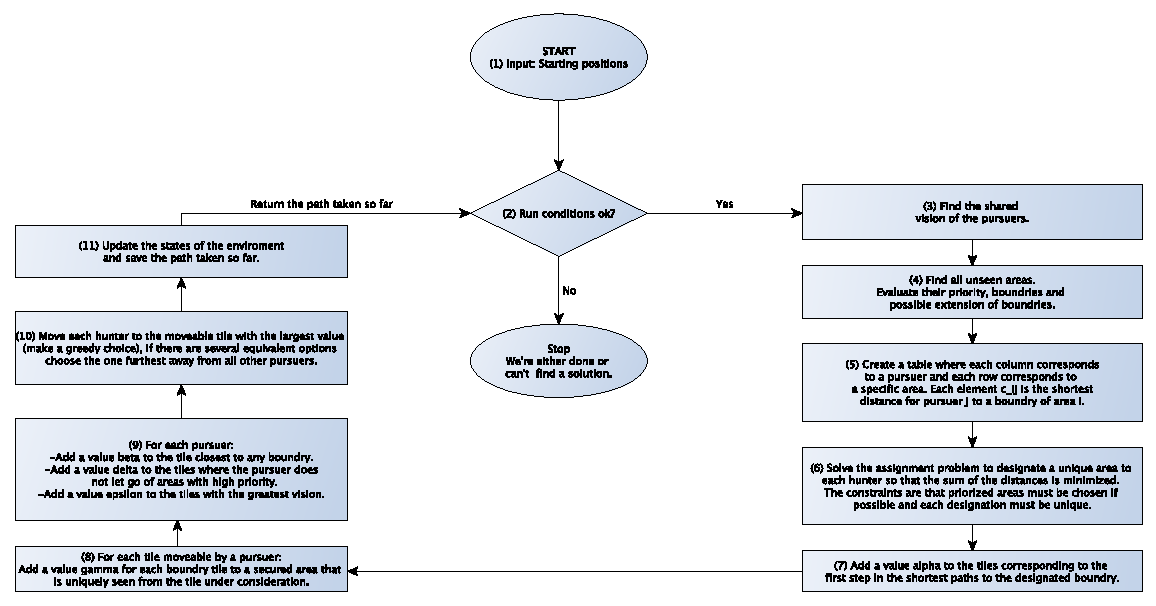
\includegraphics[width=\textwidth]{chapter_4_methods/greedy_uml4}
  	\caption[Flow chart of greedy algorithm]
  	{Flow chart of greedy algorithm}
	\label{flowchart greedy}
\end{figure}
 
In order to make a greedy choice possible it is necessary to give each tile under consideration a specific cost. At the end of an itteration the algorithm will make a greedy choice by moving each pursuer to an adjacent tile with the highest cost. The cost function will add one or several values $\alpha$, $\beta$, $\gamma$, $\delta$, $\epsilon$ to a tile depending on its geometrical and strategical properties in the current situation. The cost for a specific tile is the sum of all the parameters added to the tile. The values of the parameters $\alpha$, $\beta$, $\gamma$, $\delta$, $\epsilon$ are to be adjusted in the implementation so that the algorithm behaves properly.\\
\\The algorithm is written in an itterative way, and a overview is given by the flow chart in figure \ref{flowchart greedy} In each itteration the algorithm finds and executes the best move for each pursuer. Each step in the flowchart will be described below

\begin{enumerate}
\item{} For the first itteration the input is the starting positions of the pursuers. Later when the algorithm is running, the current position of the pursuers will be the input to each iteration.
\item{} At the beginning of each itteration a decision is made whether to make another iteration or not. An iteration should be executed if there exists tiles in enviroment that are not secured and if the breaking condition is not met. The breaking condition describes the maximum amount of iterations allowed and are given by the main program running the algorithm, so that if no solution can be found the algorithm will abort in due time. 
\item{} Here we find the total field of view of the pursuers team. This will divide the enviroment in seen and unseen areas.% as in figure 4.2.(figur som visar geometri f�r omr�den. needed??)   
\item{} All areas not visible by the pursuer team are given a priority, a boundry and if possible an extended boundry. A boundry to an area is the set of all tiles that are both adjacent to some interior tile and  also seen by some pursuer. The extended boundry to an area is the set of all tiles such that the whole area can be seen from each tile. The priority is determined by the geometric properties of the area and the state of the interior tiles of the area. If the area is secured it is only relevant to guard its boundries, thus secured areas are not to be designated in any of the preceeding steps. Contamined areas can be categorised in four different types. In descending order of priority they are:
\begin{itemize} 
\item{}Areas with only one boundry tile, where the whole area can be seen from the boundry tile.
\item{}Areas with several boundries tiles, where the whole area can be seen from some boundry tile. 
\item{}Areas with only one boundry tile, but who can not be fully seen from the boundry.
\item{}Other areas.
\end{itemize} 
\item{} In this step a table of possible choices for the pursuers is created. As mentioned above the secured areas should not be a part of the table. The extended boundries are to be used when measuring the shortest path to a boundry for a pursuer. This is because our aim is to \emph{see} the area, and the extended boundries usually provides shorter paths for the pursuers. Each row in the table corresponds to an certain area and each column corresponds to a certain pursuer. Every element in the table corresponds to the number of tiles in the shortest path for the given pursuer to a given area's boundry or extended boundry. 
\item{} Given the table created we now want to choose as many elements as there are columns, since the columns corresponds to pursuers. The choice is to be made in such a way that there is at most one element chosen from each row and column and so that the sum of the chosen elements is minimized. Also there is a constraint that the rows corresponding to areas that can be fully seen from their boundries must be chosen if possible. A chosen element $c_{i,j}$ corresponds to designating the area of row i to the pursuer of column j. If there are more pursuers than areas, an area can be designate to more than one pursuer but all areas must be designated to at least one pursuer. This is a special case of the assignment problem and can be solved for instance by the Hungarian method.
\item{} Given the designation made in the previous step, for each pursuer there is at least one path of shortest distance to the designated boundry. For each pursuer,  add a value $\alpha$ to the tiles being the first step of the paths with the shortest possible distance to the designated boundry.
\item{} By construction each pursuer has at most five feasible tiles that it can move to. For each one of these tiles, add a value $\gamma$ for every boundry tile to a secured area that is uniquely seen by this pursuer.
\item{} For each pursuer:
\begin{itemize}
\item{} Add a value $\beta$ the tile being closest to any contamined area. 
\item{} Add a value $\delta$ to the tiles where the boundries to areas that are secured, or that can be seen from its boundries, are still seen by the pursuer.
\item{} Add a value $\epsilon$ to the tiles where the pursuers has the largest field of vision.
\end{itemize}
\item{} In the previous steps we have now added at most five values to each tile in the proximity of each pursuer. For each pursuer find the tile with the largest sum and move the pursuer into this tile.
\item{} When the movement is made, update the states of the enviroment correspodingly. save the path taken so far. Return the updated states and the path taken so far to the start of the algorithm. 
\end{enumerate}
\subsection{Implementation of the greedy algorithm.}
Even though a ready-to-run implementation was not made, many parts of the implementation were finished.In the prefunction all the needed static information about the enviroment is evaluated and saved to a struct. 
\begin{verbatim}
struct Greedy{
int SolutionPath[]; 
struct Node NodeMatrix[][];
int BreakCondition[];
HashTable; 
}
\end{verbatim}
The solution path is an array where index 0 contains the number of pursuers, index 1 contains the itterations made (set to zero by the prefunction), and the rest of the indices are the coordinates for each pursuer. The NodeMatrix is the graph created by the simulation enviroment described in chapter three. The break condition is simply an integer to describe the maximum allowed itterations. Since the algorithm needs to know the distance and the path between two tiles and this is saved into a hashtable. To find the shortest path and the distance between two tiles the A-star algorithm is used. 

%FIND THE COMPLEXITY OF A-STAR!!! Dijkstra:  algorithm of $O(\vert v \vert^2)$ , a-star is special case of dijkstar? 
%pregreedy:
%a-star to find the distance and the path between any two tiles. describe complexity
%hashtable to access shortest distance in a fast manor, key: (from to)
%descride the greedy struct contents and motivate.


The implementation of the algorithm described in the previous section calls for the usage of a couple of interesting algorithms to solve some of the steps. In step four we want to find the interior of all areas. This was implemented by first taking any tile not part of the pursuers vision. Make a breadth first search to find and mark all the interior points of this area. Find a new unmarked and unseen tile and execute another breadth first search. Repeat this until all tiles not visible by the pursuer team are marked. The breadth first algorithm's time complexity is $O(\vert V \vert + \vert E \vert)$ \cite{adk8}, where V is the number of vertices in the graph and E is the number of edges.\\
\\For step six in the algorithm (the assignment) the implementation is designed to exaust all possible combinations and then pick the combination giving the smallest sum. The combinations are found by usage of a queue (first in, first out). Here one could try to use the Hungarian method \cite{hungarian} instead, but since the size of the table is usually not very large this algorithm seemed like overkill.  



